\subsection{Gaussian noise}

\Fig~\ref{fig:acc_gn_wu} displays the results obtained using altered data with gaussian noise. Specifically, \Fig~\ref{fig:gn_acc_wu_bnn} illustrates the accuracy trend of the BNN, while \Fig~\ref{fig:gaus_noise_ann} presents the trend for the standard NN. It is evident that their behavior is quite similar, although the standard ANN appears to be slightly more robust. The degradation in accuracy exhibits a linear relationship with the noise variance.

\begin{figure}[h]
	\centering
	\begin{subfigure}{.5\textwidth}
		\centering
		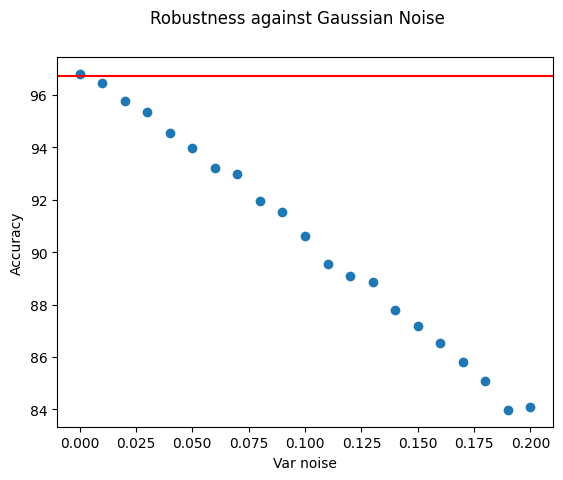
\includegraphics[width=0.8\linewidth]{ImageFiles/EvalBNN/GN/WU/acc}
		\caption{BNN}
		\label{fig:gn_acc_wu_bnn}
	\end{subfigure}%
	\begin{subfigure}{.5\textwidth}
		\centering
		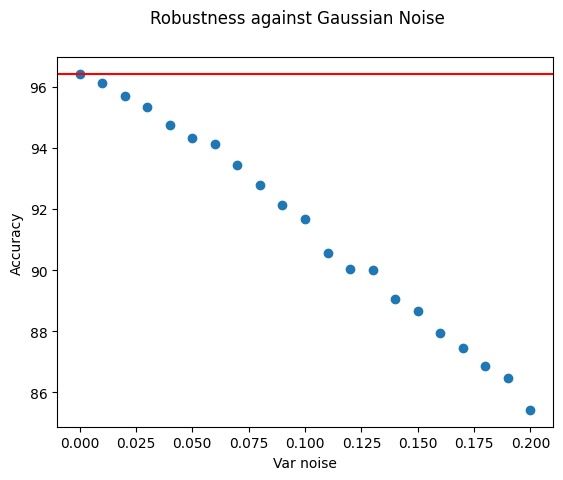
\includegraphics[width=0.8\linewidth]{ImageFiles/EvalANN/gaus_noise_ann}
		\caption{Standard NN}
		\label{fig:gaus_noise_ann}
	\end{subfigure}
	\caption{Accuracy trend for gaussian noise}
	\label{fig:acc_gn_wu}
\end{figure}

When computing robustness, the results are $0.9681$ for the BNN and $0.9740$ for the standard NN, slightly more robust than the BNN, as observed in the robustness graphs. These values are close to $1$, indicating that both networks exhibit good robustness to gaussian noise.

\Fig~\ref{fig:gn_uncertainty} shows the trend of uncertainty estimated by the BNN. In particular, \Fig~\ref{fig:gn_aleatoric} illustrates the aleatoric uncertainty trend, while \Fig~\ref{fig:gn_epistemic} presents the epistemic uncertainty.

It is worth noting that both uncertainties increase approximately linearly with respect to the noise variance. This demonstrates that input data altered with gaussian noise makes the network less certain about its predictions, and this uncertainty is linearly proportional to the noise variance.

\begin{figure}[h]
	\centering
	\begin{subfigure}{.5\textwidth}
		\centering
		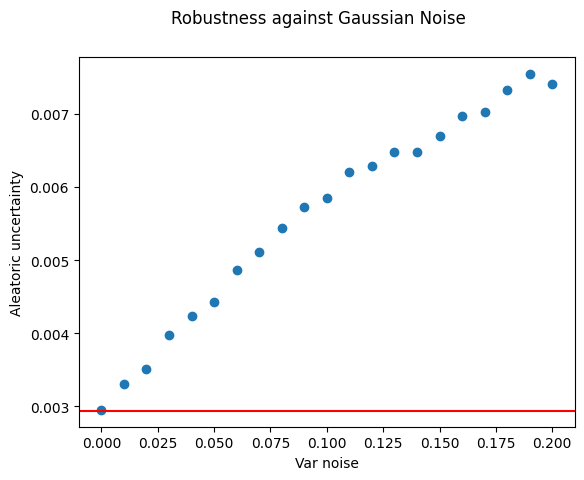
\includegraphics[width=0.8\linewidth]{ImageFiles/EvalBNN/GN/aleatoric}
		\caption{Aleatoric uncertainty}
		\label{fig:gn_aleatoric}
	\end{subfigure}%
	\begin{subfigure}{.5\textwidth}
		\centering
		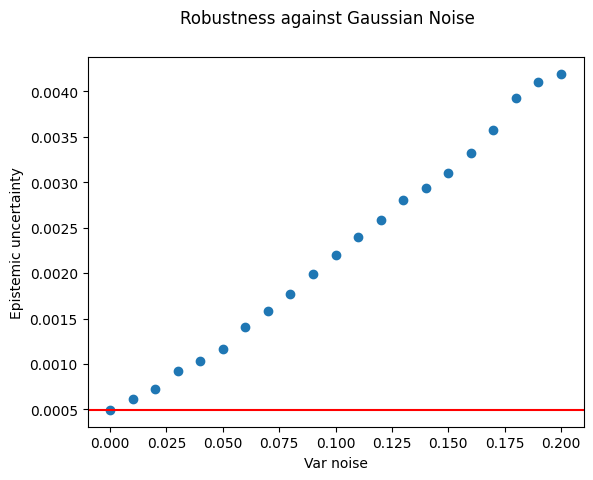
\includegraphics[width=0.8\linewidth]{ImageFiles/EvalBNN/GN/epistemic}
		\caption{Epistemic uncertainty}
		\label{fig:gn_epistemic}
	\end{subfigure}
	\caption{Uncertainty trend for gaussian noise}
	\label{fig:gn_uncertainty}
\end{figure}

The next analysis will focus on evaluating whether the estimated uncertainty utilization contributes to performance improvement.

\vspace{0.3cm}
\textbf{Classification using aleatoric uncertainty}
\vspace{0.1cm}

In \Fig~\ref{fig:gn_au}, the results of the BNN evaluation on the dataset altered with gaussian noise are illustrated, where aleatoric uncertainty is utilized as a metric to implement the ``I don't know" behavior. \Fig~\ref{fig:gn_au_acc} demonstrates that the accuracy still decreases linearly with the increase of noise variance. However, in this case, the accuracy degradation reaches a lower level. Comparing this with the case without the use of uncertainty in \Fig~\ref{fig:gn_acc_wu_bnn}, it is evident that the lowest accuracy reached is higher when uncertainty is employed.

This improvement in accuracy has a counterpart, which is the number of unknown predictions, shown in \Fig~\ref{fig:gn_au_unkn}. The unknown ratio also increases linearly with the noise variance. The same behavior is exhibited by the effectiveness, as seen in \Fig~\ref{fig:gn_au_eff}. This trend aligns with the initial analysis of aleatoric uncertainty, which was observed to increase linearly with noise variance.

\begin{figure}[h]
	\centering
	\begin{subfigure}{.33\textwidth}
		\centering
		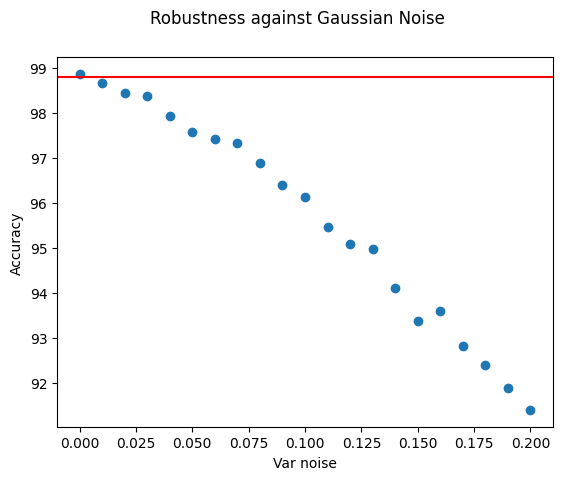
\includegraphics[width=0.9\linewidth]{ImageFiles/EvalBNN/GN/AU/acc}
		\caption{Accuracy using aleatoric \\ uncertainty}
		\label{fig:gn_au_acc}
	\end{subfigure}%
	\begin{subfigure}{.33\textwidth}
		\centering
		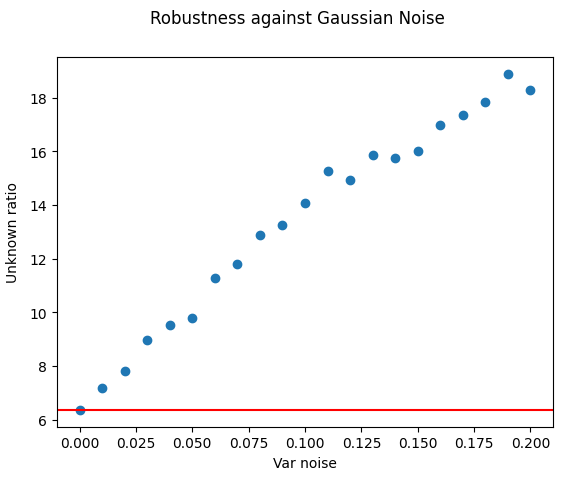
\includegraphics[width=0.9\linewidth]{ImageFiles/EvalBNN/GN/AU/unkn}
		\caption{Unknown ratio using aleatoric uncertainty}
		\label{fig:gn_au_unkn}
	\end{subfigure}%
	\begin{subfigure}{.33\textwidth}
	\centering
	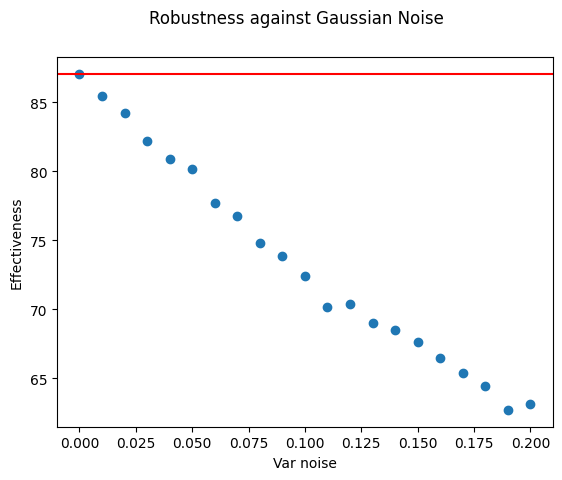
\includegraphics[width=0.9\linewidth]{ImageFiles/EvalBNN/GN/AU/eff}
	\caption{Effectiveness using aleatoric uncertainty}
	\label{fig:gn_au_eff}
	\end{subfigure}
	\caption{Robustness graph for gaussian noise when aleatoric uncertainty is employed in the classification}
	\label{fig:gn_au}
\end{figure}

\Tab~\ref{table:rob_gn_au} provides a summary of the robustness metrics resulting from this evaluation. The improvement in accuracy is reflected in the robustness, which has increased by $0.02$. It is important to interpret these values correctly because the robustness computed without uncertainty is already good, given the high accuracy values. Therefore, an improvement of $0.02$ can be considered significant in this context.

It is worth remembering that we do not penalize, and still reward, any accuracy value above $0$, as it is the minimum accepted accuracy. This is why we observe high robustness metrics. However, in this study, the specific robustness values are not the primary focus; rather, we aim to compare them among all the classification techniques.

\begin{table}[h]
	\centering
	\begin{tabular}{|| l | l ||} 
		\hline
		\textbf{Parameter} & \textbf{Value} \\
		\hline
		\hline
		$rob_{GaussianNoise}$ & $0.9842$ \\
		$robInd_{GaussianNoise}$ & $0.9624$ \\
		$robAug_{GaussianNoise}$ & $0.9217$ \\	
		\hline
	\end{tabular}	
	\caption{Robustness metrics for the gaussian noise when the aleatoric uncertainty is employed}
	\label{table:rob_gn_au}
\end{table}

To provide a meaningful interpretation of the computed metrics singularly, it is necessary to establish concrete system requirements derived from a real-world application. In this context, the tolerance and penalization functions should be fine-tuned to reflect these requirements. This will enable a more comprehensive and context-specific interpretation of the metrics.

A final observation can be made regarding the $robAug$ metric, which considers both accuracy and the unknown ratio. This provides a single integrated metric, rather than relying on two separate metrics.

\vspace{0.3cm}
\textbf{Classification using epistemic uncertainty}
\vspace{0.1cm}

Following the analysis of aleatoric uncertainty, we have examined epistemic uncertainty. \Fig~\ref{fig:gn_eu} presents the results obtained from the evaluation using this type of uncertainty.

The trend is once again linear, but there are differences in the slope. When using epistemic uncertainty, the performance in terms of the unknown ratio for low alteration levels appears to be better than in the previous case. However, this performance degrades more rapidly, ultimately reaching worse levels compared to the previous case. The accuracy trend, as shown in \Fig~\ref{fig:gn_eu_acc}, is very similar. The main difference arises in \Fig~\ref{fig:gn_eu_unkn}, where the increase in unknown predictions is more pronounced. This is better summarized by the effectiveness metric, displayed in \Fig~\ref{fig:gn_eu_eff}, which captures the behavior of the unknown ratio while also taking accuracy into account.

\begin{figure}[h]
	\centering
	\begin{subfigure}{.33\textwidth}
		\centering
		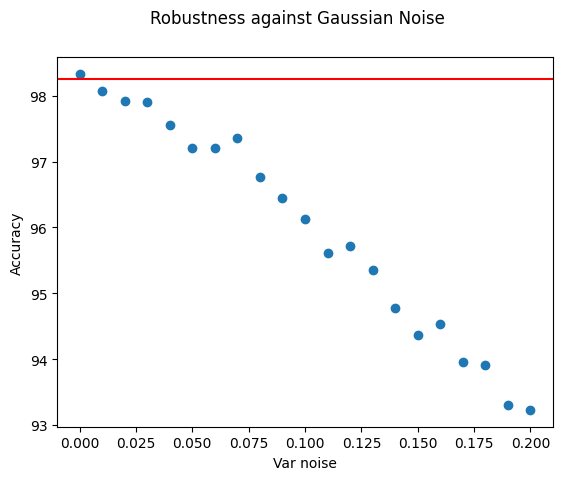
\includegraphics[width=0.9\linewidth]{ImageFiles/EvalBNN/GN/EU/acc}
		\caption{Accuracy using epistemic \\ uncertainty}
		\label{fig:gn_eu_acc}
	\end{subfigure}%
	\begin{subfigure}{.33\textwidth}
		\centering
		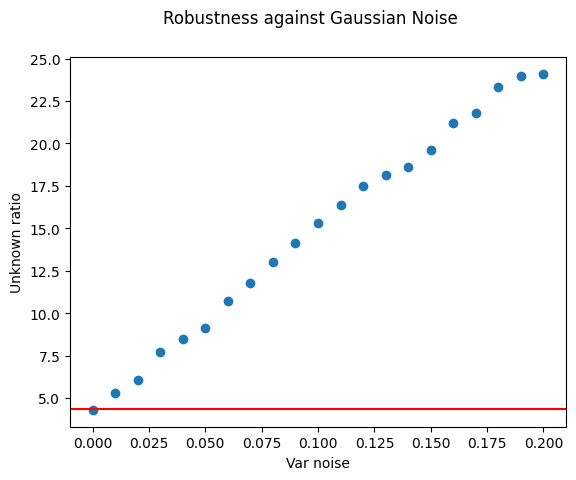
\includegraphics[width=0.9\linewidth]{ImageFiles/EvalBNN/GN/EU/unkn}
		\caption{Unknown ratio using \\ epistemic uncertainty}
		\label{fig:gn_eu_unkn}
	\end{subfigure}%
	\begin{subfigure}{.33\textwidth}
		\centering
		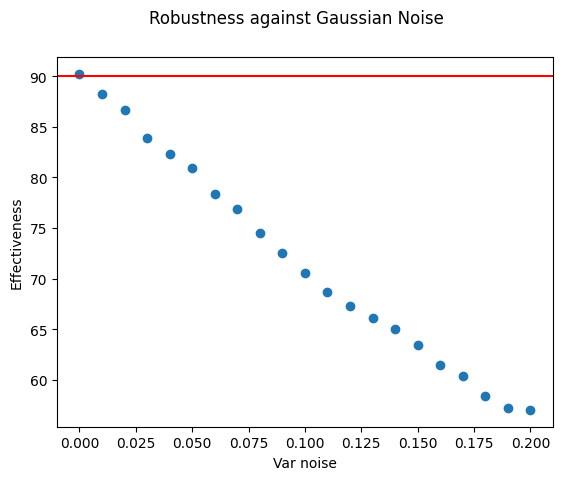
\includegraphics[width=0.9\linewidth]{ImageFiles/EvalBNN/GN/EU/eff}
		\caption{Effectiveness using \\ epistemic uncertainty}
		\label{fig:gn_eu_eff}
	\end{subfigure}
	\caption{Robustness graph for gaussian noise when epistemic uncertainty is employed in the classification}
	\label{fig:gn_eu}
\end{figure}

\Tab~\ref{table:rob_gn_eu} provides a summary of the observations made thus far. The $rob$ metric appears to have a similar value, while the other two metrics are lower than in the previous case.

\begin{table}[h]
	\centering
	\begin{tabular}{|| l | l ||} 
		\hline
		\textbf{Parameter} & \textbf{Value} \\
		\hline
		\hline
		$rob_{GaussianNoise}$ & $0.9885$ \\
		$robInd_{GaussianNoise}$ & $0.9454$ \\
		$robAug_{GaussianNoise}$ & $0.8989$ \\	
		\hline
	\end{tabular}	
	\caption{Robustness metrics for the gaussian noise when the epistemic uncertainty is employed}
	\label{table:rob_gn_eu}
\end{table}

This analysis confirms the considerations made in \Chap~\ref{chap:c3} about epistemic uncertainty, which is primarily related to the model rather than the input data. While these two concepts may be interconnected in some cases, in general, epistemic uncertainty does not directly represent characteristics of the domain data itself.

\vspace{0.3cm}
\textbf{Classification using standard deviation}
\vspace{0.1cm}

The last uncertainty type is the standard deviation, and the results are presented in \Fig~\ref{fig:gn_vu}. This evaluation exhibits higher accuracy values, as seen in \Fig~\ref{fig:gn_vu_acc}. However, the unknown ratio, shown in \Fig~\ref{fig:gn_vu_unkn}, is much higher compared to the previous two cases. This is also reflected by the effectiveness metric in \Fig~\ref{fig:gn_vu_eff}.

\begin{figure}[h]
	\centering
	\begin{subfigure}{.33\textwidth}
		\centering
		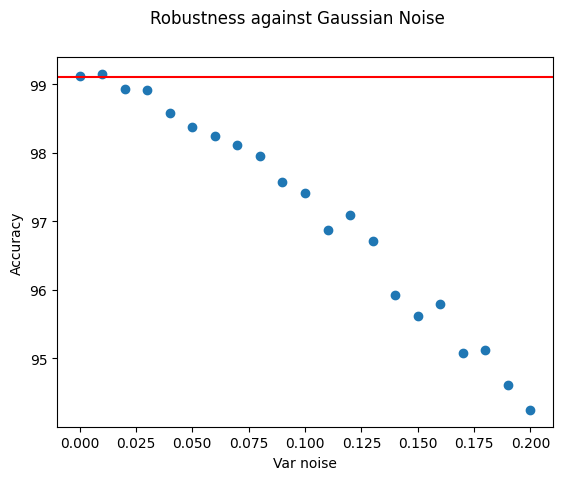
\includegraphics[width=0.9\linewidth]{ImageFiles/EvalBNN/GN/VU/acc}
		\caption{Accuracy using standard \\ deviation}
		\label{fig:gn_vu_acc}
	\end{subfigure}%
	\begin{subfigure}{.33\textwidth}
		\centering
		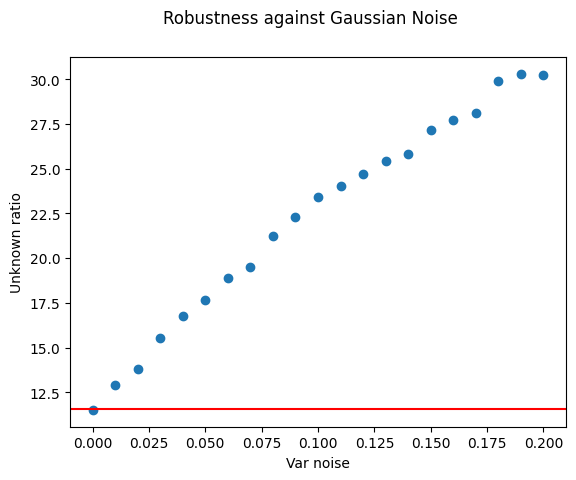
\includegraphics[width=0.9\linewidth]{ImageFiles/EvalBNN/GN/VU/unkn}
		\caption{Unknown ratio using \\ standard deviation}
		\label{fig:gn_vu_unkn}
	\end{subfigure}%
	\begin{subfigure}{.33\textwidth}
		\centering
		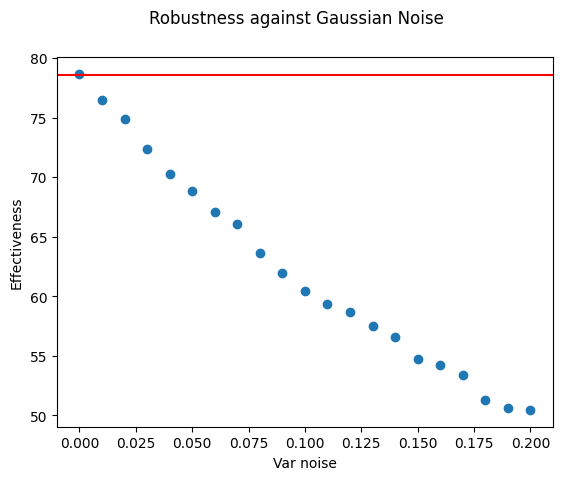
\includegraphics[width=0.9\linewidth]{ImageFiles/EvalBNN/GN/VU/eff}
		\caption{Effectiveness using standard deviation}
		\label{fig:gn_vu_eff}
	\end{subfigure}
	\caption{Robustness graph for gaussian noise when standard deviation is employed in the classification}
	\label{fig:gn_vu}
\end{figure}

\Tab~\ref{table:rob_gn_vu} provides the robustness metrics. It is worth noting that even though the unknown ratio values are higher than in the epistemic case, the two $robInd$ values are not significantly different. This is because we measure the distance from the nominal conditions and not the absolute values. In this case, the nominal unknown ratio is approximately $12\%$, which is already double the value observed in the previous cases. This could suggest that the confidence level used for this uncertainty type might be too high. As mentioned in \Chap~\ref{chap:c3}, the formula for computing the threshold is based on a linear approximation, which could lead to different behaviors among the three classification techniques.

\begin{table}[h]
	\centering
	\begin{tabular}{|| l | l ||} 
		\hline
		\textbf{Parameter} & \textbf{Value} \\
		\hline
		\hline
		$rob_{GaussianNoise}$ & $0.9900$ \\
		$robInd_{GaussianNoise}$ & $0.9392$ \\
		$robAug_{GaussianNoise}$ & $0.8954$ \\	
		\hline
	\end{tabular}	
	\caption{Robustness metrics for the gaussian noise when the standard deviation is employed}
	\label{table:rob_gn_vu}
\end{table}

\vspace{0.3cm}
\textbf{Comparison}
\vspace{0.1cm}

\Tab~\ref{table:rob_gn} provides a summary of the results obtained using the different classification methods. All methods appear to achieve an improved robustness in terms of accuracy. However, aleatoric uncertainty enables the highest robustness in terms of unknown values and effectiveness. In this particular setting, if a low degradation of the unknown ratio is desired while maintaining good accuracy, aleatoric uncertainty seems to be the most suitable choice. On the other hand, if the primary goal is to maintain a high level of accuracy, then standard deviation would be the optimal choice.

\begin{table}[h]
	\centering
	\begin{tabular}{|| l | l | l | l ||} 
		\hline
		\textbf{Parameter} & \textbf{Aleatoric} & \textbf{Epistemic} & \textbf{Standard deviation} \\
		\hline
		\hline
		$rob_{GaussianNoise}$ & $0.9842$ & $0.9885$ & $0.9900$ \\
		$robInd_{GaussianNoise}$ & $0.9624$ & $0.9454$ & $0.9392$ \\
		$robAug_{GaussianNoise}$ & $0.9217$ & $0.8989$ & $0.8954$ \\	
		\hline
	\end{tabular}	
	\caption{Summary of the robustness metrics for the gaussian noise}
	\label{table:rob_gn}
\end{table}